\documentclass{standalone}
\usepackage{tikz}
\usepackage{aeguill}
\begin{document}
% generated by Plantuml 1.2021.00      
\definecolor{plantucolor0000}{RGB}{0,0,0}
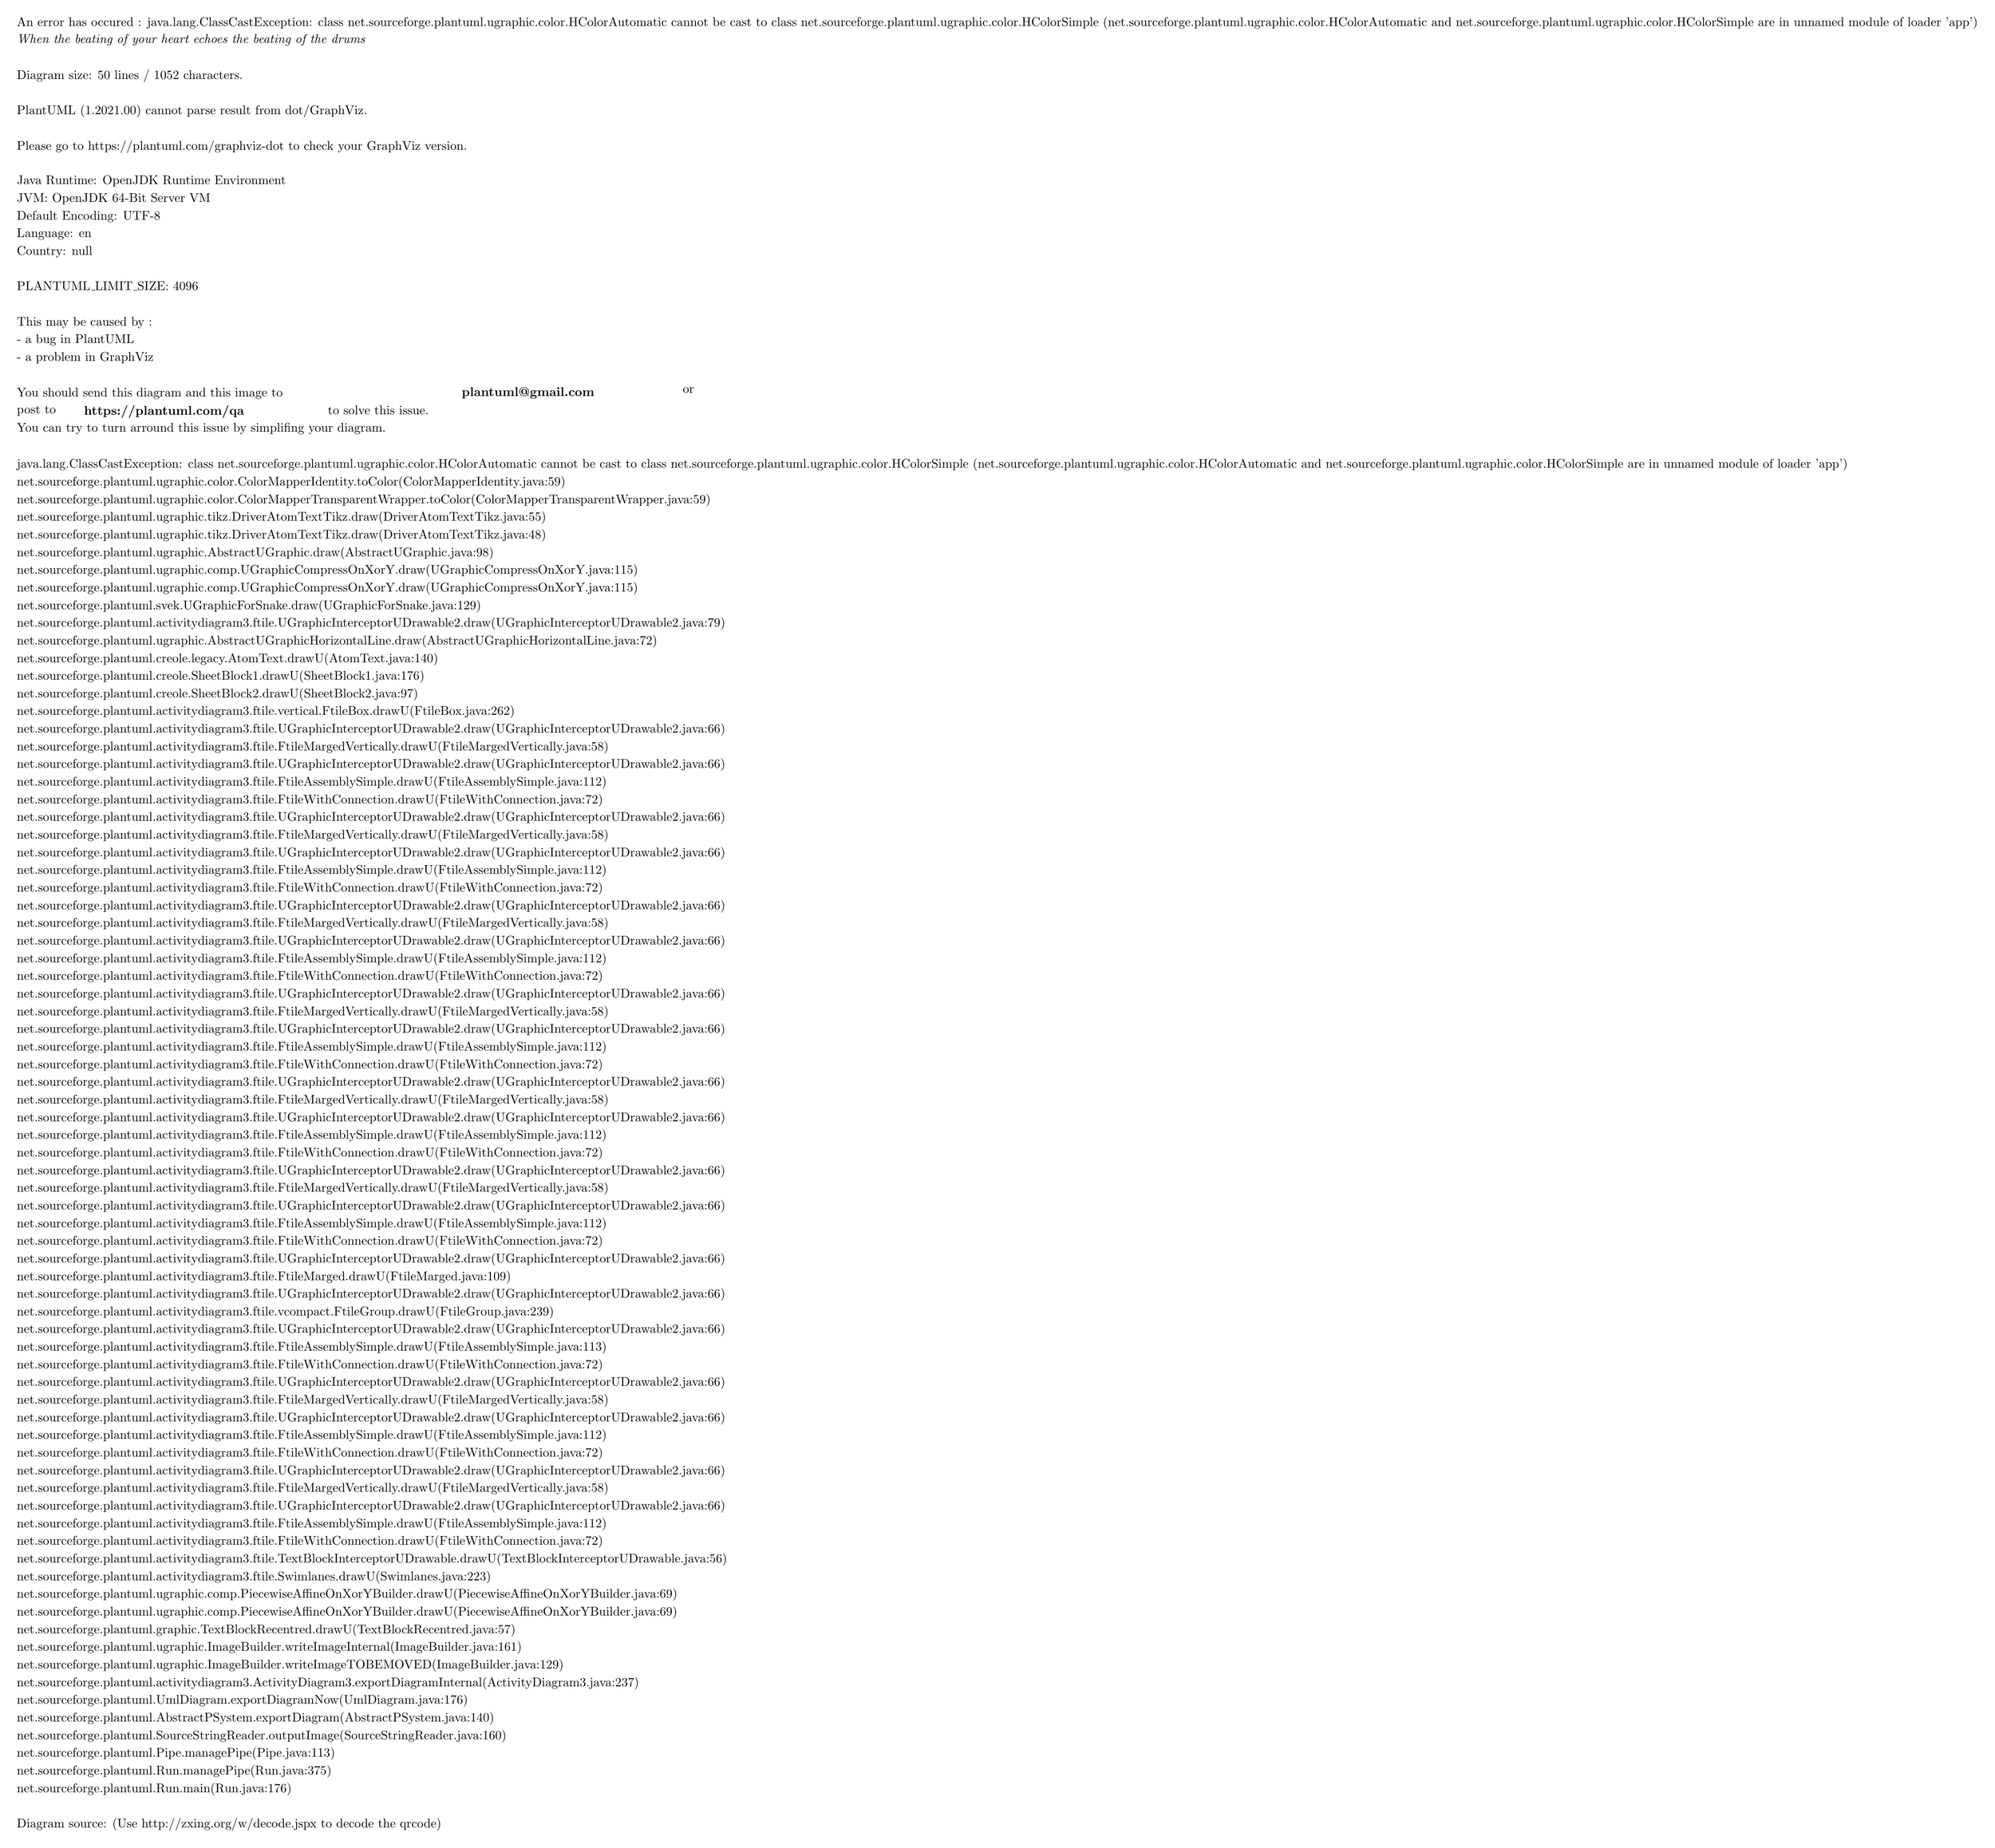
\begin{tikzpicture}[yscale=-1
]
\node at (5pt,5pt)[below right,color=black]{An error has occured : java.lang.ClassCastException: class net.sourceforge.plantuml.ugraphic.color.HColorAutomatic cannot be cast to class net.sourceforge.plantuml.ugraphic.color.HColorSimple (net.sourceforge.plantuml.ugraphic.color.HColorAutomatic and net.sourceforge.plantuml.ugraphic.color.HColorSimple are in unnamed module of loader 'app')};
\node at (5pt,18.9688pt)[below right,color=black]{\textit{When the beating of your heart echoes the beating of the drums}};
\node at (5pt,32.9375pt)[below right,color=black]{ };
\node at (5pt,46.9063pt)[below right,color=black]{Diagram size: 50 lines / 1052 characters.};
\node at (5pt,60.875pt)[below right,color=black]{ };
\node at (5pt,74.8438pt)[below right,color=black]{PlantUML (1.2021.00) cannot parse result from dot/GraphViz.};
\node at (5pt,88.8125pt)[below right,color=black]{ };
\node at (5pt,102.7813pt)[below right,color=black]{Please go to https://plantuml.com/graphviz-dot to check your GraphViz version.};
\node at (5pt,116.75pt)[below right,color=black]{ };
\node at (5pt,130.7188pt)[below right,color=black]{Java Runtime: OpenJDK Runtime Environment};
\node at (5pt,144.6875pt)[below right,color=black]{JVM: OpenJDK 64-Bit Server VM};
\node at (5pt,158.6563pt)[below right,color=black]{Default Encoding: UTF-8};
\node at (5pt,172.625pt)[below right,color=black]{Language: en};
\node at (5pt,186.5938pt)[below right,color=black]{Country: null};
\node at (5pt,200.5625pt)[below right,color=black]{ };
\node at (5pt,214.5313pt)[below right,color=black]{PLANTUML\_LIMIT\_SIZE: 4096};
\node at (5pt,228.5pt)[below right,color=black]{ };
\node at (5pt,242.4688pt)[below right,color=black]{This may be caused by :};
\node at (5pt,256.4375pt)[below right,color=black]{ - a bug in PlantUML};
\node at (5pt,270.4063pt)[below right,color=black]{ - a problem in GraphViz};
\node at (5pt,284.375pt)[below right,color=black]{ };
\node at (5pt,298.4727pt)[below right,color=black]{You should send this diagram and this image to };
\node at (356.88pt,298.3438pt)[below right,color=black]{\textbf{plantuml@gmail.com}};
\node at (531.6692pt,298.4727pt)[below right,color=black]{ or};
\node at (5pt,312.5703pt)[below right,color=black]{post to };
\node at (58.113pt,312.4414pt)[below right,color=black]{\textbf{https://plantuml.com/qa}};
\node at (251.0221pt,312.5703pt)[below right,color=black]{ to solve this issue.};
\node at (5pt,326.5391pt)[below right,color=black]{You can try to turn arround this issue by simplifing your diagram.};
\node at (5pt,340.5078pt)[below right,color=black]{ };
\node at (5pt,354.4766pt)[below right,color=black]{java.lang.ClassCastException: class net.sourceforge.plantuml.ugraphic.color.HColorAutomatic cannot be cast to class net.sourceforge.plantuml.ugraphic.color.HColorSimple (net.sourceforge.plantuml.ugraphic.color.HColorAutomatic and net.sourceforge.plantuml.ugraphic.color.HColorSimple are in unnamed module of loader 'app')};
\node at (5pt,368.4453pt)[below right,color=black]{  net.sourceforge.plantuml.ugraphic.color.ColorMapperIdentity.toColor(ColorMapperIdentity.java:59)};
\node at (5pt,382.4141pt)[below right,color=black]{  net.sourceforge.plantuml.ugraphic.color.ColorMapperTransparentWrapper.toColor(ColorMapperTransparentWrapper.java:59)};
\node at (5pt,396.3828pt)[below right,color=black]{  net.sourceforge.plantuml.ugraphic.tikz.DriverAtomTextTikz.draw(DriverAtomTextTikz.java:55)};
\node at (5pt,410.3516pt)[below right,color=black]{  net.sourceforge.plantuml.ugraphic.tikz.DriverAtomTextTikz.draw(DriverAtomTextTikz.java:48)};
\node at (5pt,424.3203pt)[below right,color=black]{  net.sourceforge.plantuml.ugraphic.AbstractUGraphic.draw(AbstractUGraphic.java:98)};
\node at (5pt,438.2891pt)[below right,color=black]{  net.sourceforge.plantuml.ugraphic.comp.UGraphicCompressOnXorY.draw(UGraphicCompressOnXorY.java:115)};
\node at (5pt,452.2578pt)[below right,color=black]{  net.sourceforge.plantuml.ugraphic.comp.UGraphicCompressOnXorY.draw(UGraphicCompressOnXorY.java:115)};
\node at (5pt,466.2266pt)[below right,color=black]{  net.sourceforge.plantuml.svek.UGraphicForSnake.draw(UGraphicForSnake.java:129)};
\node at (5pt,480.1953pt)[below right,color=black]{  net.sourceforge.plantuml.activitydiagram3.ftile.UGraphicInterceptorUDrawable2.draw(UGraphicInterceptorUDrawable2.java:79)};
\node at (5pt,494.1641pt)[below right,color=black]{  net.sourceforge.plantuml.ugraphic.AbstractUGraphicHorizontalLine.draw(AbstractUGraphicHorizontalLine.java:72)};
\node at (5pt,508.1328pt)[below right,color=black]{  net.sourceforge.plantuml.creole.legacy.AtomText.drawU(AtomText.java:140)};
\node at (5pt,522.1016pt)[below right,color=black]{  net.sourceforge.plantuml.creole.SheetBlock1.drawU(SheetBlock1.java:176)};
\node at (5pt,536.0703pt)[below right,color=black]{  net.sourceforge.plantuml.creole.SheetBlock2.drawU(SheetBlock2.java:97)};
\node at (5pt,550.0391pt)[below right,color=black]{  net.sourceforge.plantuml.activitydiagram3.ftile.vertical.FtileBox.drawU(FtileBox.java:262)};
\node at (5pt,564.0078pt)[below right,color=black]{  net.sourceforge.plantuml.activitydiagram3.ftile.UGraphicInterceptorUDrawable2.draw(UGraphicInterceptorUDrawable2.java:66)};
\node at (5pt,577.9766pt)[below right,color=black]{  net.sourceforge.plantuml.activitydiagram3.ftile.FtileMargedVertically.drawU(FtileMargedVertically.java:58)};
\node at (5pt,591.9453pt)[below right,color=black]{  net.sourceforge.plantuml.activitydiagram3.ftile.UGraphicInterceptorUDrawable2.draw(UGraphicInterceptorUDrawable2.java:66)};
\node at (5pt,605.9141pt)[below right,color=black]{  net.sourceforge.plantuml.activitydiagram3.ftile.FtileAssemblySimple.drawU(FtileAssemblySimple.java:112)};
\node at (5pt,619.8828pt)[below right,color=black]{  net.sourceforge.plantuml.activitydiagram3.ftile.FtileWithConnection.drawU(FtileWithConnection.java:72)};
\node at (5pt,633.8516pt)[below right,color=black]{  net.sourceforge.plantuml.activitydiagram3.ftile.UGraphicInterceptorUDrawable2.draw(UGraphicInterceptorUDrawable2.java:66)};
\node at (5pt,647.8203pt)[below right,color=black]{  net.sourceforge.plantuml.activitydiagram3.ftile.FtileMargedVertically.drawU(FtileMargedVertically.java:58)};
\node at (5pt,661.7891pt)[below right,color=black]{  net.sourceforge.plantuml.activitydiagram3.ftile.UGraphicInterceptorUDrawable2.draw(UGraphicInterceptorUDrawable2.java:66)};
\node at (5pt,675.7578pt)[below right,color=black]{  net.sourceforge.plantuml.activitydiagram3.ftile.FtileAssemblySimple.drawU(FtileAssemblySimple.java:112)};
\node at (5pt,689.7266pt)[below right,color=black]{  net.sourceforge.plantuml.activitydiagram3.ftile.FtileWithConnection.drawU(FtileWithConnection.java:72)};
\node at (5pt,703.6953pt)[below right,color=black]{  net.sourceforge.plantuml.activitydiagram3.ftile.UGraphicInterceptorUDrawable2.draw(UGraphicInterceptorUDrawable2.java:66)};
\node at (5pt,717.6641pt)[below right,color=black]{  net.sourceforge.plantuml.activitydiagram3.ftile.FtileMargedVertically.drawU(FtileMargedVertically.java:58)};
\node at (5pt,731.6328pt)[below right,color=black]{  net.sourceforge.plantuml.activitydiagram3.ftile.UGraphicInterceptorUDrawable2.draw(UGraphicInterceptorUDrawable2.java:66)};
\node at (5pt,745.6016pt)[below right,color=black]{  net.sourceforge.plantuml.activitydiagram3.ftile.FtileAssemblySimple.drawU(FtileAssemblySimple.java:112)};
\node at (5pt,759.5703pt)[below right,color=black]{  net.sourceforge.plantuml.activitydiagram3.ftile.FtileWithConnection.drawU(FtileWithConnection.java:72)};
\node at (5pt,773.5391pt)[below right,color=black]{  net.sourceforge.plantuml.activitydiagram3.ftile.UGraphicInterceptorUDrawable2.draw(UGraphicInterceptorUDrawable2.java:66)};
\node at (5pt,787.5078pt)[below right,color=black]{  net.sourceforge.plantuml.activitydiagram3.ftile.FtileMargedVertically.drawU(FtileMargedVertically.java:58)};
\node at (5pt,801.4766pt)[below right,color=black]{  net.sourceforge.plantuml.activitydiagram3.ftile.UGraphicInterceptorUDrawable2.draw(UGraphicInterceptorUDrawable2.java:66)};
\node at (5pt,815.4453pt)[below right,color=black]{  net.sourceforge.plantuml.activitydiagram3.ftile.FtileAssemblySimple.drawU(FtileAssemblySimple.java:112)};
\node at (5pt,829.4141pt)[below right,color=black]{  net.sourceforge.plantuml.activitydiagram3.ftile.FtileWithConnection.drawU(FtileWithConnection.java:72)};
\node at (5pt,843.3828pt)[below right,color=black]{  net.sourceforge.plantuml.activitydiagram3.ftile.UGraphicInterceptorUDrawable2.draw(UGraphicInterceptorUDrawable2.java:66)};
\node at (5pt,857.3516pt)[below right,color=black]{  net.sourceforge.plantuml.activitydiagram3.ftile.FtileMargedVertically.drawU(FtileMargedVertically.java:58)};
\node at (5pt,871.3203pt)[below right,color=black]{  net.sourceforge.plantuml.activitydiagram3.ftile.UGraphicInterceptorUDrawable2.draw(UGraphicInterceptorUDrawable2.java:66)};
\node at (5pt,885.2891pt)[below right,color=black]{  net.sourceforge.plantuml.activitydiagram3.ftile.FtileAssemblySimple.drawU(FtileAssemblySimple.java:112)};
\node at (5pt,899.2578pt)[below right,color=black]{  net.sourceforge.plantuml.activitydiagram3.ftile.FtileWithConnection.drawU(FtileWithConnection.java:72)};
\node at (5pt,913.2266pt)[below right,color=black]{  net.sourceforge.plantuml.activitydiagram3.ftile.UGraphicInterceptorUDrawable2.draw(UGraphicInterceptorUDrawable2.java:66)};
\node at (5pt,927.1953pt)[below right,color=black]{  net.sourceforge.plantuml.activitydiagram3.ftile.FtileMargedVertically.drawU(FtileMargedVertically.java:58)};
\node at (5pt,941.1641pt)[below right,color=black]{  net.sourceforge.plantuml.activitydiagram3.ftile.UGraphicInterceptorUDrawable2.draw(UGraphicInterceptorUDrawable2.java:66)};
\node at (5pt,955.1328pt)[below right,color=black]{  net.sourceforge.plantuml.activitydiagram3.ftile.FtileAssemblySimple.drawU(FtileAssemblySimple.java:112)};
\node at (5pt,969.1016pt)[below right,color=black]{  net.sourceforge.plantuml.activitydiagram3.ftile.FtileWithConnection.drawU(FtileWithConnection.java:72)};
\node at (5pt,983.0703pt)[below right,color=black]{  net.sourceforge.plantuml.activitydiagram3.ftile.UGraphicInterceptorUDrawable2.draw(UGraphicInterceptorUDrawable2.java:66)};
\node at (5pt,997.0391pt)[below right,color=black]{  net.sourceforge.plantuml.activitydiagram3.ftile.FtileMarged.drawU(FtileMarged.java:109)};
\node at (5pt,1011.0078pt)[below right,color=black]{  net.sourceforge.plantuml.activitydiagram3.ftile.UGraphicInterceptorUDrawable2.draw(UGraphicInterceptorUDrawable2.java:66)};
\node at (5pt,1024.9766pt)[below right,color=black]{  net.sourceforge.plantuml.activitydiagram3.ftile.vcompact.FtileGroup.drawU(FtileGroup.java:239)};
\node at (5pt,1038.9453pt)[below right,color=black]{  net.sourceforge.plantuml.activitydiagram3.ftile.UGraphicInterceptorUDrawable2.draw(UGraphicInterceptorUDrawable2.java:66)};
\node at (5pt,1052.9141pt)[below right,color=black]{  net.sourceforge.plantuml.activitydiagram3.ftile.FtileAssemblySimple.drawU(FtileAssemblySimple.java:113)};
\node at (5pt,1066.8828pt)[below right,color=black]{  net.sourceforge.plantuml.activitydiagram3.ftile.FtileWithConnection.drawU(FtileWithConnection.java:72)};
\node at (5pt,1080.8516pt)[below right,color=black]{  net.sourceforge.plantuml.activitydiagram3.ftile.UGraphicInterceptorUDrawable2.draw(UGraphicInterceptorUDrawable2.java:66)};
\node at (5pt,1094.8203pt)[below right,color=black]{  net.sourceforge.plantuml.activitydiagram3.ftile.FtileMargedVertically.drawU(FtileMargedVertically.java:58)};
\node at (5pt,1108.7891pt)[below right,color=black]{  net.sourceforge.plantuml.activitydiagram3.ftile.UGraphicInterceptorUDrawable2.draw(UGraphicInterceptorUDrawable2.java:66)};
\node at (5pt,1122.7578pt)[below right,color=black]{  net.sourceforge.plantuml.activitydiagram3.ftile.FtileAssemblySimple.drawU(FtileAssemblySimple.java:112)};
\node at (5pt,1136.7266pt)[below right,color=black]{  net.sourceforge.plantuml.activitydiagram3.ftile.FtileWithConnection.drawU(FtileWithConnection.java:72)};
\node at (5pt,1150.6953pt)[below right,color=black]{  net.sourceforge.plantuml.activitydiagram3.ftile.UGraphicInterceptorUDrawable2.draw(UGraphicInterceptorUDrawable2.java:66)};
\node at (5pt,1164.6641pt)[below right,color=black]{  net.sourceforge.plantuml.activitydiagram3.ftile.FtileMargedVertically.drawU(FtileMargedVertically.java:58)};
\node at (5pt,1178.6328pt)[below right,color=black]{  net.sourceforge.plantuml.activitydiagram3.ftile.UGraphicInterceptorUDrawable2.draw(UGraphicInterceptorUDrawable2.java:66)};
\node at (5pt,1192.6016pt)[below right,color=black]{  net.sourceforge.plantuml.activitydiagram3.ftile.FtileAssemblySimple.drawU(FtileAssemblySimple.java:112)};
\node at (5pt,1206.5703pt)[below right,color=black]{  net.sourceforge.plantuml.activitydiagram3.ftile.FtileWithConnection.drawU(FtileWithConnection.java:72)};
\node at (5pt,1220.5391pt)[below right,color=black]{  net.sourceforge.plantuml.activitydiagram3.ftile.TextBlockInterceptorUDrawable.drawU(TextBlockInterceptorUDrawable.java:56)};
\node at (5pt,1234.5078pt)[below right,color=black]{  net.sourceforge.plantuml.activitydiagram3.ftile.Swimlanes.drawU(Swimlanes.java:223)};
\node at (5pt,1248.4766pt)[below right,color=black]{  net.sourceforge.plantuml.ugraphic.comp.PiecewiseAffineOnXorYBuilder.drawU(PiecewiseAffineOnXorYBuilder.java:69)};
\node at (5pt,1262.4453pt)[below right,color=black]{  net.sourceforge.plantuml.ugraphic.comp.PiecewiseAffineOnXorYBuilder.drawU(PiecewiseAffineOnXorYBuilder.java:69)};
\node at (5pt,1276.4141pt)[below right,color=black]{  net.sourceforge.plantuml.graphic.TextBlockRecentred.drawU(TextBlockRecentred.java:57)};
\node at (5pt,1290.3828pt)[below right,color=black]{  net.sourceforge.plantuml.ugraphic.ImageBuilder.writeImageInternal(ImageBuilder.java:161)};
\node at (5pt,1304.3516pt)[below right,color=black]{  net.sourceforge.plantuml.ugraphic.ImageBuilder.writeImageTOBEMOVED(ImageBuilder.java:129)};
\node at (5pt,1318.3203pt)[below right,color=black]{  net.sourceforge.plantuml.activitydiagram3.ActivityDiagram3.exportDiagramInternal(ActivityDiagram3.java:237)};
\node at (5pt,1332.2891pt)[below right,color=black]{  net.sourceforge.plantuml.UmlDiagram.exportDiagramNow(UmlDiagram.java:176)};
\node at (5pt,1346.2578pt)[below right,color=black]{  net.sourceforge.plantuml.AbstractPSystem.exportDiagram(AbstractPSystem.java:140)};
\node at (5pt,1360.2266pt)[below right,color=black]{  net.sourceforge.plantuml.SourceStringReader.outputImage(SourceStringReader.java:160)};
\node at (5pt,1374.1953pt)[below right,color=black]{  net.sourceforge.plantuml.Pipe.managePipe(Pipe.java:113)};
\node at (5pt,1388.1641pt)[below right,color=black]{  net.sourceforge.plantuml.Run.managePipe(Run.java:375)};
\node at (5pt,1402.1328pt)[below right,color=black]{  net.sourceforge.plantuml.Run.main(Run.java:176)};
\node at (5pt,1416.1016pt)[below right,color=black]{ };
\node at (5pt,1430.0703pt)[below right,color=black]{ Diagram source: (Use http://zxing.org/w/decode.jspx to decode the qrcode)};
\end{tikzpicture}
\end{document}
